\documentclass[11pt]{article}
\usepackage[utf8]{inputenc}
\usepackage[T1]{fontenc}
\usepackage{amsmath}
\usepackage{multicol}
\usepackage{geometry}
\usepackage{tikz}
\usetikzlibrary{shapes.geometric, arrows.meta, calc}
\usepackage{enumitem}
\usepackage{xcolor}
\usepackage{titlesec}

% Configurações de layout
\geometry{a4paper, left=1cm, right=1cm, top=0.5cm, bottom=1.2cm}
\setlength{\columnseprule}{0.4pt}
\setlength{\baselineskip}{1.0\baselineskip}

% Cores personalizadas
\definecolor{titleblue}{RGB}{0,80,150}
\definecolor{sectionred}{RGB}{180,0,0}
\definecolor{darkgreen}{RGB}{0,100,0}

% Formatação de títulos
\titleformat{\section}{\normalfont\Large\bfseries\color{titleblue}}{\thesection}{1em}{}
\titleformat{\subsection}{\normalfont\large\bfseries\color{sectionred}}{\thesubsection}{1em}{}
\titleformat{\subsubsection}{\normalfont\normalsize\bfseries\color{darkgreen}}{\thesubsubsection}{1em}{}

\title{\textcolor{titleblue}{Domínio e Imagem de Funções}}
\author{Professor: Jefferson}
\date{}

\begin{document}

\maketitle
\vspace{-1cm}

\begin{center}
\large{Nome: \underline{\hspace{8cm}} \quad Turma: \underline{\hspace{3cm}}}
\end{center}

\begin{multicols}{2}

\section*{1. Conjuntos Numéricos Fundamentais}

\subsection*{1.1 Números Naturais ($\mathbb{N}$)}
\begin{itemize}
    \item Contagem natural: $\{1, 2, 3, \dots\}$
    \item Alguns incluem o zero: $\{0, 1, 2, \dots\}$
    \item Representação:
    \begin{center}
    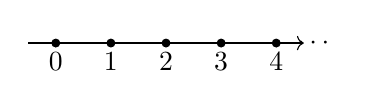
\begin{tikzpicture}[scale=0.7]
        \draw[->] (-0.5,0) -- (4.5,0);
        \foreach \x in {0,1,2,3,4} {
            \filldraw (\x,0) circle (2pt) node[below] {$\x$};
        }
        \node at (4.2,0) [right] {$\cdots$};
    \end{tikzpicture}
    \end{center}
\end{itemize}

\subsection*{1.2 Números Inteiros ($\mathbb{Z}$)}
\begin{itemize}
    \item Inclui negativos: $\{\dots, -2, -1, 0, 1, 2, \dots\}$
    \item Representação:
    \begin{center}
    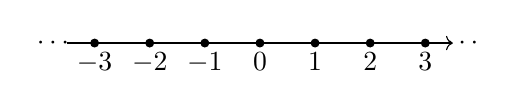
\begin{tikzpicture}[scale=0.7]
        \draw[->] (-3.5,0) -- (3.5,0);
        \foreach \x in {-3,-2,-1,0,1,2,3} {
            \filldraw (\x,0) circle (2pt) node[below] {$\x$};
        }
        \node at (3.2,0) [right] {$\cdots$};
        \node at (-3.2,0) [left] {$\cdots$};
    \end{tikzpicture}
    \end{center}
\end{itemize}

\subsection*{1.3 Números Racionais ($\mathbb{Q}$)}
\begin{itemize}
    \item Frações $\frac{a}{b}$ onde $b \neq 0$
    \item Exemplos: $\frac{1}{2}$, $-\frac{3}{4}$, $0,333...$
    \item Podem ser representados como decimais finitos ou periódicos
    \item Representação:
    \begin{center}
    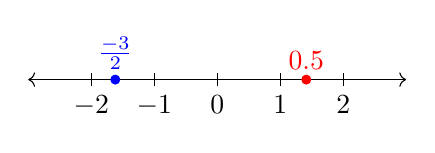
\begin{tikzpicture}[scale=0.8]
        \draw[<->] (-3,0) -- (3,0);
        \foreach \x in {-2,-1,0,1,2} {
            \draw (\x,0.1) -- (\x,-0.1) node[below] {$\x$};
        }
        \filldraw[red] (1.414,0) circle (2pt) node[above] {$0.5$};
        \filldraw[blue] (-1.618,0) circle (2pt) node[above] {$\frac{-3}{2}$};
    \end{tikzpicture}
    \end{center}
\end{itemize}

\subsection*{1.4 Números Reais ($\mathbb{R}$)}
\begin{itemize}
    \item Inclui todos os racionais e irracionais
    \item Exemplos de irracionais: $\sqrt{2}$, $\pi$, $e$
    \item Reta real contínua:
    \begin{center}
    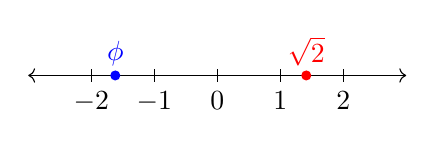
\begin{tikzpicture}[scale=0.8]
        \draw[<->] (-3,0) -- (3,0);
        \foreach \x in {-2,-1,0,1,2} {
            \draw (\x,0.1) -- (\x,-0.1) node[below] {$\x$};
        }
        \filldraw[red] (1.414,0) circle (2pt) node[above] {$\sqrt{2}$};
        \filldraw[blue] (-1.618,0) circle (2pt) node[above] {$\phi$};
    \end{tikzpicture}
    \end{center}
\end{itemize}


\subsection*{Relação entre Conjuntos Numéricos}
\begin{center}
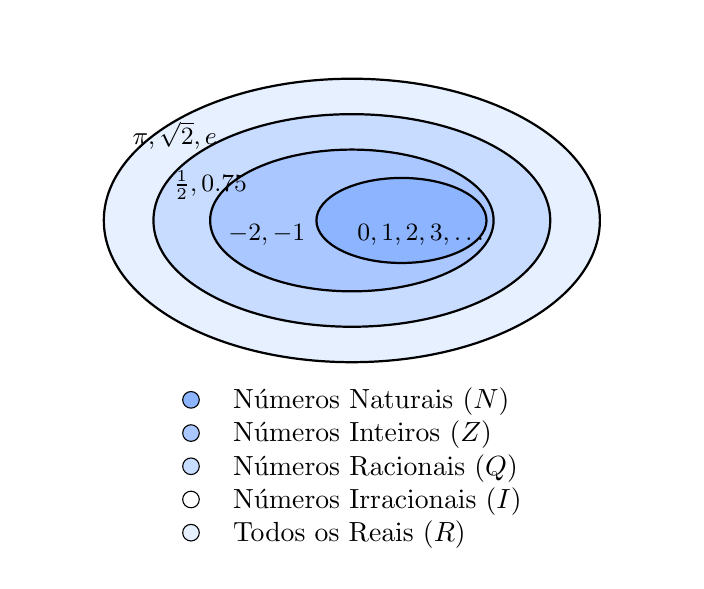
\begin{tikzpicture}[scale=0.9]
    % Configuração de cores
    \definecolor{outercolor}{RGB}{230,240,255}
    \definecolor{middlecolor}{RGB}{200,220,255}
    \definecolor{innercolor}{RGB}{170,200,255}
    \definecolor{corecolor}{RGB}{140,180,255}
    
    % Conjunto dos Reais
    \draw[fill=outercolor, thick] (0,0) ellipse (3.5 and 2) node[above, yshift=2.2cm] {};
    
    % Conjunto dos Racionais
    \draw[fill=middlecolor, thick] (0,0) ellipse (2.8 and 1.5) node {\large $\mathbb{Q}$};
    \node at (3.5,0.5) {};
    
    % Conjunto dos Inteiros
    \draw[fill=innercolor, thick] (0,0) ellipse (2 and 1) node {\large $\mathbb{Z}$};
    
    % Conjunto dos Naturais
    \draw[fill=corecolor, thick] (0.7,0) ellipse (1.2 and 0.6) node {};
    
    % Legenda Hierárquica
    \node at (0,-3.5) [text width=8cm, align=center] {
        \begin{tabular}{cl}
            \tikz\draw[fill=corecolor] (0,0) circle (0.3em); & Números Naturais ($\mathbb{N}$) \\
            \tikz\draw[fill=innercolor] (0,0) circle (0.3em); & Números Inteiros ($\mathbb{Z}$) \\
            \tikz\draw[fill=middlecolor] (0,0) circle (0.3em); & Números Racionais ($\mathbb{Q}$) \\
            \tikz\draw[fill=white] (0,0) circle (0.3em); & Números Irracionais ($\mathbb{I}$) \\
            \tikz\draw[fill=outercolor] (0,0) circle (0.3em); & Todos os Reais ($\mathbb{R}$)
        \end{tabular}
    };
    
    % Exemplos
    \node at (-2.5,1.2) {\small $\pi, \sqrt{2}, e$};
    \node at (-2.0,0.5) {\small $\frac{1}{2}, 0.75$};
    \node at (-1.2,-0.2) {\small $-2, -1$};
    \node at (1.0,-0.2) {\small $0, 1, 2, 3, \dots$};
\end{tikzpicture}
\end{center}

\section*{2. Domínio de uma Função}

\subsection*{2.1 Conceito}
O domínio (D) é o conjunto de todos os valores de entrada (x) para os quais a função está definida.


\subsection*{Exemplos Detalhados}
\begin{enumerate}
    \item $f(x) = 2x + 3$ \\
    \textit{Domínio}: $\mathbb{R}$ (qualquer x real é válido)
    
    \item $g(x) = \dfrac{1}{x-4}$ \\
    \textit{Restrição}: $x-4 \neq 0 \Rightarrow x \neq 4$ \\
    \textit{Domínio}: $\mathbb{R} - \{4\}$
    
    \item $h(x) = \sqrt{x+5}$ \\
    \textit{Restrição}: $x+5 \geq 0 \Rightarrow x \geq -5$ \\
    \textit{Domínio}: $[-5, +\infty)$
\end{enumerate}

\section*{2. Imagem de uma Função}
A imagem (Im) é o conjunto de \textbf{todos os valores de saída} (y) que a função pode produzir.

\subsection*{Como determinar?}
\begin{itemize}
    \item \textbf{Funções do 1º grau}: $Im = \mathbb{R}$
    \item \textbf{Funções quadráticas}: Analisar vértice
    \item \textbf{Funções raiz}: $y \geq 0$ (para índice par)
    \item \textbf{Funções exponenciais}: $y > 0$
\end{itemize}

\begin{center}
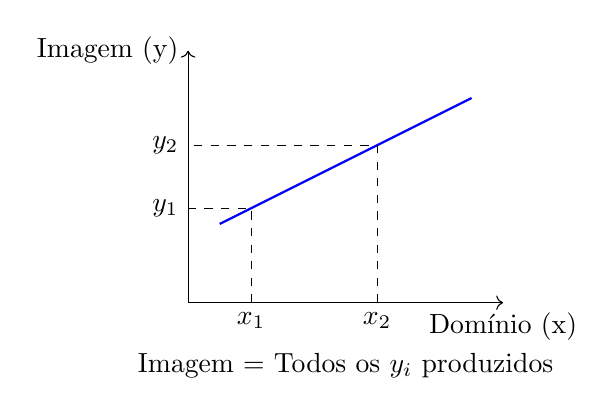
\begin{tikzpicture}[scale=0.8]
    % Função
    \draw[->] (0,0) -- (5,0) node[below] {Domínio (x)};
    \draw[->] (0,0) -- (0,4) node[left] {Imagem (y)};
    % Curva
    \draw[blue, thick, domain=0.5:4.5] plot (\x, {0.5*\x + 1});
    % Projeção
    \draw[dashed] (1,0) node[below] {$x_1$} -- (1,1.5) -- (0,1.5) node[left] {$y_1$};
    \draw[dashed] (3,0) node[below] {$x_2$} -- (3,2.5) -- (0,2.5) node[left] {$y_2$};
    % Legenda
    \node at (2.5,-1) {Imagem = Todos os $y_i$ produzidos};
\end{tikzpicture}
\end{center}

\subsection*{Exemplos Detalhados}
\begin{enumerate}
    \item $f(x) = x^2$ \\
    \textit{Imagem}: $[0, +\infty)$ (quadrados são sempre não-negativos)
    
    \item $g(x) = -3x + 2$ \\
    \textit{Imagem}: $\mathbb{R}$ (funções lineares cobrem todos os reais)
    
    \item $h(x) = 2^x$ \\
    \textit{Imagem}: $(0, +\infty)$ (exponencial sempre positiva)
\end{enumerate}

\section*{3. Diagrama de Máquina}
Uma analogia útil para entender domínio e imagem:

\begin{center}
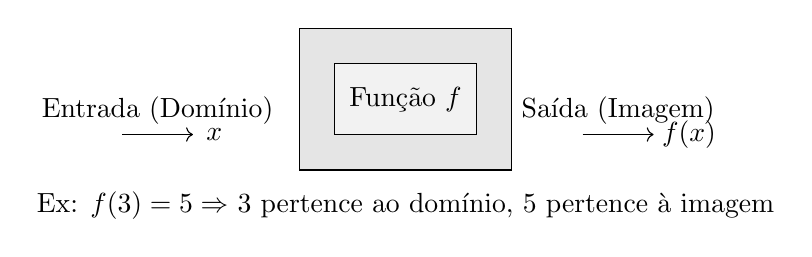
\begin{tikzpicture}[scale=0.9]
    % Máquina
    \draw[fill=gray!20] (1,0) rectangle (4,2);
    \draw[fill=gray!10] (1.5,0.5) rectangle (3.5,1.5);
    \node at (2.5,1) {Função $f$};
    % Entrada
    \draw[->] (-1.5,0.5) -- (-0.5,0.5) node[midway,above] {Entrada (Domínio)};
    \node at (-0.2,0.5) {$x$};
    % Saída
    \draw[->] (5,0.5) -- (6,0.5) node[midway,above] {Saída (Imagem)};
    \node at (6.5,0.5) {$f(x)$};
    % Exemplo
    \node at (2.5,-0.5) {Ex: $f(3) = 5 \Rightarrow$ 3 pertence ao domínio, 5 pertence à imagem};
\end{tikzpicture}
\end{center}

\section*{4. Exercícios Básicos (1-10)}
\begin{enumerate}
    \item Determine o domínio das funções:
    \begin{enumerate}[label=\alph*)]
        \item $f(x) = 5x - 2$
        \item $g(x) = \dfrac{x+1}{x-3}$
        \item $h(x) = \sqrt{2x - 6}$
    \end{enumerate}
    
    \item Determine a imagem das funções:
    \begin{enumerate}[label=\alph*)]
        \item $f(x) = x^2 + 4$
        \item $g(x) = -2x + 5$
        \item $h(x) = \sqrt{9 - x^2}$
    \end{enumerate}
    
    \item Classifique como verdadeiro (V) ou falso (F):
    \begin{enumerate}[label=\alph*)]
        \item ( ) O domínio de $f(x) = \dfrac{1}{x}$ é $\mathbb{R}$
        \item ( ) A imagem de $f(x) = |x|$ é $[0, +\infty)$
        \item ( ) $\sqrt{x^2} = x$ para todo $x \in \mathbb{R}$
    \end{enumerate}
    
    \item Associe cada função ao seu domínio:
    \begin{enumerate}[label=\alph*)]
        \item $f(x) = \dfrac{1}{\sqrt{x}}$ \hspace{0.5cm} ( ) $x > 0$
        \item $g(x) = \log(x+2)$ \hspace{0.5cm} ( ) $x \neq 0$
        \item $h(x) = \dfrac{x}{x^2-4}$ \hspace{0.5cm} ( ) $x > -2$
    \end{enumerate}
    
    \item Resolva:
    \begin{enumerate}[label=\alph*)]
        \item Para $f(x) = \sqrt{4-x}$, calcule $f(0)$, $f(4)$ e $f(5)$
        \item Qual o maior domínio possível para $f(x) = \dfrac{1}{\sqrt{x-1}}$?
    \end{enumerate}
\end{enumerate}

\section*{5. Exercícios Intermediários (11-20)}
\begin{enumerate}\setcounter{enumi}{5}
    \item Esboce o gráfico e determine D e Im:
    \begin{enumerate}[label=\alph*)]
        \item $f(x) = x^2 - 4$
        \item $g(x) = \dfrac{1}{x+2}$
    \end{enumerate}
    
    \item Determine o domínio máximo de:
    \begin{enumerate}[label=\alph*)]
        \item $f(x) = \dfrac{\sqrt{x}}{x^2-9}$
        \item $g(x) = \log(x^2 - 4)$
    \end{enumerate}
    
    \item Problemas aplicados:
    \begin{enumerate}[label=\alph*)]
        \item A área de um círculo é $A(r) = \pi r^2$. Determine D e Im considerando $r$ como raio.
        \item O volume de uma caixa cúbica é $V(a) = a^3$. Determine D e Im considerando $a$ como aresta.
    \end{enumerate}
    
    \item Funções definidas por partes:
    \begin{enumerate}[label=\alph*)]
        \item $f(x) = \begin{cases} x+2, & x < 1 \\ 5, & x \geq 1 \end{cases}$. Determine D e Im.
    \end{enumerate}
    
    \item Desafio:
    \begin{enumerate}[label=\alph*)]
        \item Determine o domínio de $f(x) = \sqrt{\dfrac{x-2}{x+3}}$
        \item Determine a imagem de $f(x) = \dfrac{x}{x^2+1}$
    \end{enumerate}
\end{enumerate}

\subsection*{Gabarito Sugerido}
\begin{tabular}{|c|l|c|l|}
\hline
\textbf{Questão} & \textbf{Resposta} & \textbf{Questão} & \textbf{Resposta} \\
\hline
1a) & $\mathbb{R}$ & 11a) & D = $\mathbb{R}$, Im = $[-4,+\infty)$ \\
1b) & $\mathbb{R} - \{3\}$ & 11b) & D = $\mathbb{R} - \{-2\}$, Im = $\mathbb{R} - \{0\}$ \\
1c) & $x \geq 3$ & 12a) & $x \geq 0$ e $x \neq \pm 3$ \\
2a) & $[4,+\infty)$ & 12b) & $x < -2$ ou $x > 2$ \\
2b) & $\mathbb{R}$ & 13a) & D = $(0,+\infty)$, Im = $(0,+\infty)$ \\
2c) & $[0,3]$ & 13b) & D = $(0,+\infty)$, Im = $(0,+\infty)$ \\
3a) & F & 14a) & D = $\mathbb{R}$, Im = $(-\infty,3) \cup \{5\}$ \\
3b) & V & 15a) & $x \leq -3$ ou $x \geq 2$ \\
3c) & F & 15b) & $[-\frac{1}{2},\frac{1}{2}]$ \\
4a) & (1) & & \\
4b) & (3) & & \\
4c) & (2) & & \\
\hline
\end{tabular}

\end{multicols}

\end{document}
